% Options for packages loaded elsewhere
\PassOptionsToPackage{unicode}{hyperref}
\PassOptionsToPackage{hyphens}{url}
%
\documentclass[
  12pt,
]{article}
\usepackage{lmodern}
\usepackage{amssymb,amsmath}
\usepackage{ifxetex,ifluatex}
\ifnum 0\ifxetex 1\fi\ifluatex 1\fi=0 % if pdftex
  \usepackage[T1]{fontenc}
  \usepackage[utf8]{inputenc}
  \usepackage{textcomp} % provide euro and other symbols
\else % if luatex or xetex
  \usepackage{unicode-math}
  \defaultfontfeatures{Scale=MatchLowercase}
  \defaultfontfeatures[\rmfamily]{Ligatures=TeX,Scale=1}
\fi
% Use upquote if available, for straight quotes in verbatim environments
\IfFileExists{upquote.sty}{\usepackage{upquote}}{}
\IfFileExists{microtype.sty}{% use microtype if available
  \usepackage[]{microtype}
  \UseMicrotypeSet[protrusion]{basicmath} % disable protrusion for tt fonts
}{}
\makeatletter
\@ifundefined{KOMAClassName}{% if non-KOMA class
  \IfFileExists{parskip.sty}{%
    \usepackage{parskip}
  }{% else
    \setlength{\parindent}{0pt}
    \setlength{\parskip}{6pt plus 2pt minus 1pt}}
}{% if KOMA class
  \KOMAoptions{parskip=half}}
\makeatother
\usepackage{xcolor}
\IfFileExists{xurl.sty}{\usepackage{xurl}}{} % add URL line breaks if available
\IfFileExists{bookmark.sty}{\usepackage{bookmark}}{\usepackage{hyperref}}
\hypersetup{
  hidelinks,
  pdfcreator={LaTeX via pandoc}}
\urlstyle{same} % disable monospaced font for URLs
\usepackage[margin=1in]{geometry}
\usepackage{graphicx}
\makeatletter
\def\maxwidth{\ifdim\Gin@nat@width>\linewidth\linewidth\else\Gin@nat@width\fi}
\def\maxheight{\ifdim\Gin@nat@height>\textheight\textheight\else\Gin@nat@height\fi}
\makeatother
% Scale images if necessary, so that they will not overflow the page
% margins by default, and it is still possible to overwrite the defaults
% using explicit options in \includegraphics[width, height, ...]{}
\setkeys{Gin}{width=\maxwidth,height=\maxheight,keepaspectratio}
% Set default figure placement to htbp
\makeatletter
\def\fps@figure{htbp}
\makeatother
\setlength{\emergencystretch}{3em} % prevent overfull lines
\providecommand{\tightlist}{%
  \setlength{\itemsep}{0pt}\setlength{\parskip}{0pt}}
\setcounter{secnumdepth}{-\maxdimen} % remove section numbering
\usepackage{booktabs}
\usepackage{longtable}
\usepackage{array}
\usepackage{multirow}
\usepackage{wrapfig}
\usepackage{float}
\usepackage{colortbl}
\usepackage{pdflscape}
\usepackage{tabu}
\usepackage{threeparttable}
\usepackage{threeparttablex}
\usepackage[normalem]{ulem}
\usepackage{makecell}
\usepackage{caption}
\usepackage{hyperref}
\usepackage{helvet} % Helvetica font
\renewcommand*\familydefault{\sfdefault} % Use the sans serif version of the font
\usepackage[T1]{fontenc}
\usepackage[labelfont=bf]{caption}

\usepackage[none]{hyphenat}

\usepackage{setspace}
\doublespacing
\setlength{\parskip}{1em}

\usepackage{lineno}

\usepackage{pdfpages}
\floatplacement{figure}{H} % Keep the figure up top of the page
\DeclareUnicodeCharacter{0301}{*************************************}
\newlength{\cslhangindent}
\setlength{\cslhangindent}{1.5em}
\newenvironment{cslreferences}%
  {}%
  {\par}

\author{}
\date{\vspace{-2.5em}}

\begin{document}

\pagenumbering{arabic}
\linenumbers
\doublespacing

\hypertarget{the-gut-microbiota-potentiates-clostridiodes-difficile-infection-severity.}{%
\section{\texorpdfstring{The gut microbiota potentiates
\emph{Clostridiodes difficile} infection
severity.}{The gut microbiota potentiates Clostridiodes difficile infection severity.}}\label{the-gut-microbiota-potentiates-clostridiodes-difficile-infection-severity.}}

\vspace{30mm}

\textbf{Running title:} Microbiota potentiates \emph{Clostridioides
difficile} infection severity

\vspace{20mm}

Nicholas A. Lesniak\(^1\), Alyxandria M. Schubert\(^1\), Kaitlyn
Flynn\(^1\), Hamide Sinani\(^1\), Kathyrn A. Eaton\(^1\), Ingrid L.
Bergin\(^2\), Patrick D. Schloss\(^{1,\dagger}\)

\vspace{30mm}

\(\dagger\) To whom correspondence should be addressed:
\href{mailto:pschloss@umich.edu}{\nolinkurl{pschloss@umich.edu}}\\
1. Department of Microbiology and Immunology, University of Michigan,
Ann Arbor, MI\\
2. Unit for Laboratory Animal Medicine, University of Michigan, Ann
Arbor, MI

\newpage

\hypertarget{abstract}{%
\subsection{Abstract}\label{abstract}}

\emph{Clostridioides difficile} infection has become more common and
severe in the last few decades. Patient age, white blood cell count,
creatinine levels as well as \emph{C. difficile} ribotype and the
presence of toxin genes have been associated with disease severity.
However, models based on those data to identify patients with CDI that
will develop severe disease have not been robust enough to be broadly
applied. These models are input from our understanding of \emph{C.
difficile} interactions with the gut environment. The gut bacteria are a
key determinant in \emph{C. difficile} infection. CDI is dependent on
perturbations in the bacterial community in order to colonize the gut.
The gut microbiota also impairs \emph{C. difficile} colonization through
bile acid metabolism, nutrient consumption and bacteriocin production.
However, it is unclear if the gut bacteria affect the disease severity
resulting from that colonization. Here we have shown gut bacterial
communities contribute to disease severity variation. We created diverse
gut communities by colonizing germ-free mice with human fecal
communities. They were then infected with \emph{C. difficile} which
resulted in differed disease severities. The severity grouped by the
human fecal community they received. Generally, facultative anaerobes
with pathogenic potential, such as Escherichia, Helicobacter and
Klebsiella, were associated with more severe disease. Bacterial groups
associated with dietary fiber degradation, such as Coprobacillus, were
associated with reduced disease severity. Lastly, we showed communities
that resulted in either low or high histopathologic scores or severe
disease had the same outcome when infected with a different \emph{C.
difficile} isolate.

\hypertarget{importance}{%
\subsection{Importance}\label{importance}}

Clostridioides difficile infection (CDI) causes a range of disease from
asymptomatic to mild diarrhea to severe outcomes of recurrent infections
and even death. Models that predict severity and treatment decisions are
based on clinical factors and \emph{C. difficile} capabilities. But
currently the gut microbiome, the primary protector against CDI, has not
been accounted for its effect on CDI disease severity. We demonstrated
variation in the microbiome of mice colonized with human feces was
sufficient to result in a range of disease severities. Our results show
groups of bacteria contribute to the development of disease in \emph{C.
difficile} infections. Gut bacterial community data from patients with
CDI could improve our ability to identify patients more at risk for
severe disease and improve interventions which treat the gut bacteria to
reduce host damage.

\newpage

\hypertarget{introduction}{%
\subsection{Introduction}\label{introduction}}

\emph{Clostridioides difficile} infections (CDI) have been increasing in
incidence and severity since \emph{C. difficile} was first identified as
a pathogen. It was first identified in 1931 in a healthy fecal community
{[}CITATION{]}. But then in the late 1970s, following the introduction
of broad-spectrum antibiotics, \emph{C. difficile} was identified as the
cause of antibiotic-associated psuedomembranous colitis {[}CITATION{]}.
Beginning in the early 2000s, CDI became more problematic with
increasing incidences and severity {[}CITATION{]}. Disease severities
can range from asymptomatic to mild diarrhea to toxic megacolon and
death. This severity has been associated with characteristics of
\emph{C. difficile} ribotypes and host factors. Over time more
pathogenic ribotypes have emerged, such as ribotype 027 in the early
2000s. The presence of the genes for Toxin A/B or fluoroquinolon
resistence has been associated with more severe disease {[}CITATION{]}.
Binary toxin, while alone insufficient to cause damage on it own, when
in the presence of Toxin A/B has been associated with increased
virulence {[}CITATION{]}. Mutations in tcd C, the negative regulator of
of toxin transcription, also increased the virulence of \emph{C.
difficile} {[}CITATION{]}. In addition to the pathogenic potential of
the infecting strain, the response by the host also affects the disease
severity. Delayed or reduced production of antibodies IgG and IgA can
result in more severe disease {[}CITATION{]}. Increased neutrophil
inflitration can lead to worse outcomes {[}CITATION{]}. In addition to
the immune response, increased density of the toxin receptor on the host
cells can increase the severity of the infection {[}CITATION{]}. While
there is a thorough understanding of many of the mechanisms driving in
CDI incidence and disease severity, there still is not effective tools
to reduce the risk of severe disease.

Models have been developed to identify patients at risk for severe CDI
but have not been robust for broad application (1). These models utilize
patient related data, such as patient age, white blood cell count, serum
albumin levels, and creatinine levels, to predict disease severity. In
their initial publication, these models perform well enough for
publication. However when Perry et al applied many of the most current
models to a multi-center external validation, their performance suffered
and often had more false positives than true positives (3). Thus, there
seems to be a missing factor contributing to disease severity.

Missing from these models are the gut bacteria which also interact with
\emph{C. difficile} during the course of the infection. The indigenous
bacteria of a healthy intestinal community provide a protective barrier
preventing \emph{C. difficile} from infecting the gut. Only after this
community is disrupted from a range of pertubations, such as many
classes of antibiotics, medications, or even dietary changes, can
\emph{C. difficile} infect the intestine. Once established, the gut
bacteria can either promote or inhibit \emph{C. difficile} through
producing molecules or modifying the environment {[}Abbas2020{]}. Bile
acids metabolized by the gut bacteria can inhibit \emph{C. difficile}
growth and affect toxin production (5). Bacteria in the gut also can
compete more directly with \emph{C. difficile} through antibiotic
production or nutrient consumption (7). To eliminate CDI, the primary
treatment is a course of antibiotics. Patients who become reinfected and
recalitrant to antibiotics, a fecal microbiota transplantion often is
sufficient to restore the gut community to eliminate \emph{C.
difficile}. While there has been many studies to investigate the
interaction between the gut bacteria and \emph{C. difficile} during the
infection, it has not been demostrated the bacterial community can
modulate the disease severity of CDI. Recently, Tomkovich et al showed
the variation in the bacterial communtiies between mice from different
colonies and vendors was sufficient to cause differences in the temporal
dynamics of the \emph{C. difficile} infection (9). Since the gut
bacteria interact with \emph{C. difficile} throughout the infection and
community difference resulted in different colonization dynamics, we
hypothesized that the gut bacteria contribute to the variation in CDI
disease severity. Here, we colonized germ-free C57BL/6 mice with human
fecal communities to test if the variablity in the gut bacteria can
produce and explain variation in the disease severity caused by a single
\emph{C. difficile} isolate.

\hypertarget{results}{%
\subsection{Results}\label{results}}

\textbf{Germ-free mice colonized with human fecal commmunities have
diverse and unique community structures.} Based on our previous
observation mice with variation in their microbiota showed differences
in colonization of \emph{C. difficile} (9), we sought to explore the
effect communties with greater variation had on \emph{C. difficile}
challenge. To produce communities with greater variation than mouse
colonies with their indigenous communties, we used human fecal
communities to establish a community in the intestine of germ-free mice.
We inoculated a cage of germ-free C57BL/6 mice (2-4 mice per cage) with
homogenized feces from one of 15 different human donors via oral gavage.
The fecal community was allowed to colonize and stabilize for two weeks
post inoculation {[}CITATION?{]}. We then assessed the gut bacterial
communities by sequencing the V4 region of the 16S rRNA gene extracted
from fecal pellets (Figure 1A). The communities established in the mice
group most closely to other mice recieving the same human fecal donor
community than to either their respective donor or any mice who received
stool from a different donor (Figure 1B). Most of the communities were
primairily composed of populations of \emph{Clostridia},
\emph{Bacteroidia}, \emph{Erysipelotrichia}, \emph{Bacilli}, and
\emph{Gammaproteobacteria}. However, each group of mice harbored unique
combination of class abunadances in their gut bacterial communities.
\emph{Any alpha? compare to murine variation? Number of unique otus?}

\textbf{\emph{C. difficile} is able to colonize mice without
perturbation.} Our goal was to test the effect of the variation in the
microbiota on \emph{C. difficile} infection. A typical mouse model of
CDI requires pretreatment with antibiotics such as clindamycin to become
susceptible to \emph{C. difficile} colonization {[}CITATION{]}. However,
we wanted to avoid modifying the communties with an antibiotic to
maintain their community structures and differences. Since these
communties came from human donors which may have become susceptible
through their own exposures, we decided to test if \emph{C. difficile}
was able to colonize these communities without any perturbation. After
two weeks post incoluation with human fecal communities, the mice were
then challenged with 10\^{}\textbf{4?} \emph{C. difficile} ribotype 027
isolate 431 spores (\textbf{Add schematic?}) (10). The mice were
followed for 10 days post challenge and their stool was collected and
plated for \emph{C. difficile} CFU to detect colonization level. We
hypothesized that \emph{C. difficile} would most likely be able to
colonize the mice with communities that came from donors which had a
history of antibiotic use, one of the primary risk factors for
developing CDI (TABLE, CITATION). Suprisingly, communities from all
donors were colonized (Figure 2). The only two mice that were able to
resist \emph{C. difficile} colonization both recieved their community
from the same donor. Therefore, the transplanted human fecal communties
were susceptible to \emph{C. difficile} colonization without the need
for any perturbation.

\textbf{Infection seveity varies by initial community structure.} After
challenging the mice with \emph{C. difficile}, we looked at the effect
of the community variation on the outcome from the \emph{C. difficile}
infection. We followed the mice for signs of disease as well as \emph{C.
difficile} colonization and toxin production for 10 days post challenge.
Some mice were not initally colonized on the day after \emph{C.
difficile} challenge but became colonized with a few days post challenge
(\textbf{SUPP FIG?}). A subset of mice, all that recieved their comunity
from one of 6 donors, suffered from severe disease, which became highly
colonized one day post challenge and moribund within 3 days post
challenge. The remaining mice, except for one cage, maintained \emph{C.
difficile} colonization through the end of the experiment (Figure 2).
After the mice were humanely euthanised at the endpoint, day 10 post
challenge or earlier if they became moribund, their cecal tissue was
collected and scored for histological signs of disease and fecal samples
were assayed for toxin (Figure 3). Overall, there was greater toxin
activity detected in the stool of the moribund mice (\emph{P} = 0.003).
However, when looking at each group of mice, we saw there was a range in
toxin activity for both the mice with non-severe disease and severe
disease (Figure 3A). Some donor groups that maintained colonization
without severe disease had similarlly high activity levels as was
detected in the mice with severe disease. Additionally, some mice with
severe disease did not have toxin activity detected in their stool.
These oberserved variations in toxin activity and relation to disease
severity have been previously characterized (11). Next we examined the
cecal tissue for histopathological damage. For mice with severe disease,
we observed high levels of epithelial damage, tissue edema and
inflammation (Figure SXXXX), similar to previously reported
histopathologic findings for \emph{C. difficile} ribotype 027 (13). As
observed with toxin activity, the mice with severe disease had higher
histopathologic scores than the mice with non-severe disease (\emph{P} =
3.0e-9). However, unlike the toxin activity, all moribund mice had
consistently high histopathologic scores. The mice which maintained
persistent population size, we saw a range in tissue damage from no
signs of disease to nearly the same level as the mice with severe
disease, which grouped by community donor. Together, the toxin activity,
histopathologic score, and moribundity showed variation across the
donors but were largely consistent within each group of mice recieving
the same human donor fecal community.

\textbf{Populations of the microbial communities explain variation in
CDI disease severity.} Since the disease charateristics grouped by human
donor fecal community, we next investigated the community composition
for its ability to explain the variation in disease severity. First, we
tested for associations between taxonomic groups and the outcomes of the
\emph{C. difficile} infection. We used the linear discriminant analysis
(LDA) effect size (LEfSe) method to identify differences in the genera
of the initial bacterial communities between the severity level and
toxin production. We split the mice into groups by severity level based
on their if they became moribund (severe), or if their clinical score
was above 5 (moderate) or below 5 (mild). This analysis revealed 20
genera that were significantly different by the disease severity (Figure
4A). The presence of populations of \emph{Turicibacter},
\emph{Streptococcus}, \emph{Staphylococcus}, \emph{Pseudomonas},
\emph{Phocaeicola}, \emph{Parabacteroides}, \emph{Bacteroides}, and
\emph{Escherichia/Shigella} were detected at higher levels in the mice
that developed severe disease. Populations of \emph{Anaerotignum},
\emph{Coprobacillus}, \emph{Enterocloster}, and \emph{Murimonas} were
increased in the mice that would experience mild disease. There were
many genera that did not have a correlation of relative abundance and
disease severity, such as the populations of \emph{Monoglobus} and
\emph{Hungatella}, which were decreased or increased, respectively, in
only the group of mice that would develop moderate disease. To
understand these cases better we used LEfSe to identify the genera
differentiating the communities that we detected toxin in from those
that we did not (Figure 4B). There were many genera the were associated
with toxin production as we would expect from their association with
severe disease, such as populations of \emph{Escherichia/Shigella} and
\emph{Bacteroides}. Likewise, there were genera such as
\emph{Anaerotignum}, \emph{Enterocloster}, and \emph{Murimonas} that
were higher in communities that had mild disease and no toxin was
produced. However, communities without a linear trend between relative
abundance and disease severity can be better understood by their
association with toxin production. Populations of \emph{Hungatella} were
increased in the group with moderate disease but not with the production
of toxin. Lastly, we looked for associations between the histopathologic
score and the populations of genera at that same time (Figure 4C). The
populatons of \emph{Bacteroides} at the end matched the trend observed
in the initial community, increased population correlated with increased
histopathologic score. Populations of \emph{Klebsiella} and
\emph{Prevotellaceae} positively correlated with clinic score and were
increased in the group that produced toxin. These tests have identified
which individual populations of bacteria that associated with each
disease severity.

We next wanted to understand how the populations in the context of each
other lead to the different disease severities. We trained random forest
models with the intital bacterial community relative abundance data at
each taxonomic rank to predict toxin production, severe disease or final
histopathologic score. Overall for predicting toxin production,
microbial populations aggregated by their phylum level classificiation
performed as well as models using lower taxonomic ranks (AUROC = 0.83,
Figure S2). In the initial community populations of
\emph{Verrucomicrobia}, \emph{Campilobacterota} and
\emph{Proteobacteria} contributed the most to the correct prediction of
toxin production (Figure 5A). \emph{C. difficile} was more likely to
produce toxin when the initial community had smaller populations of
\emph{Verrucomicrobia} and \emph{Campilobacterota} and had larger
popluations of \emph{Proteobacteria}. Next, we assessed the ability of
the community to predict severe disease. Class rank classification was
sufficient to predict if the mouse would succumb to the infection before
the end of the experiment (AUROC = 0.91, Figure S2). Groups of bacteria
belonging to \emph{Bacilli}, \emph{Firmicutes}, and
\emph{Erysipelotrichia} contributed the most to the correct prediction.
Larger populations of \emph{Bacilli} and \emph{Firmicutes} and reduced
populations of \emph{Erysipelotrichia} were more likely to result in
moribundity (Figure 5B). Aside from \emph{Erysipelotrichia}, the only
other population decreased in moribund mice was \emph{Clostridia}, all
other features had increased populations in the moribund mice. Lastly,
the initial community was able to predict if the mice would have a
histopathologic score above or below the median score (median
histopathologic score = 5) with the genera relative abundances (AUROC =
0.99, Figure S2). There were no genera with a significantly greater
effect on the model performance than any others, indicating the model is
reliant on many genera for the correct prediction. The model used some
of the genera identified in the LEfSe analysis, such as populations of
\emph{Coprobacillus}, \emph{Anaerostipes}, and \emph{Hungatella}.
Communities with greater populations of \emph{Hungatella},
\emph{Eggerthella}, \emph{Bifidobacterium}, \emph{Duncaniella} and
\emph{Neisseria} were more likely to have greater histopathologic
scores.

\textbf{Disease severity consistent by donor community across
strains/isolates.} We used a single \emph{C. difficile} isolate,
ribotype 027 isolate 431 to characterize the range of disease severity
and the features of the bacterial community associated with severity
(10). Since we had used the same mice and \emph{C. difficile} isolate in
our first set of experiemnts, we next wanted to test if the effect of
the community would apply to other \emph{C. difficile} isolates. We
selected three communities based on the result from our analysis thus
far to select one community we would expect to result in a low clinical
score (\textless{} 5), a high clinical score (\textgreater{} 5), and one
with a high clinical score which becomes moribund. Using genus level
data to select the communities, we selected communities based on the
relative abundance patterns of \emph{Sellimonas} and \emph{Anaerotignum}
(higher abundance in mice with a low clinical score),
\emph{Lachnospiracea} (lower abundance in moribund mice),
\emph{Hungatella} and \emph{Eisenbergiella} (higher abundance in
moderate mice and lower in moribund mice), Clostridium sensu stricto
(higher in moribund mice by both LEfSe analysis and RF model) and
\emph{Enterocloster} (lower in moribund mice and a negative linear trend
with disease severity by LEfSe analysis) (Figure S3). With this set of
human fecal communities selected, we inoculated mice via oral gavage of
the human fecal slurry and allowed two weeks for the a community to
establish. We then challenged the mice with a different \emph{C.
difficile} (10). The disease severity for this set of experiments
closely matched that in our first set of experiments with \emph{C.
difficile} isolate 431 (Figure 6).

\hypertarget{discussion}{%
\subsection{Discussion}\label{discussion}}

Challenging mice colonized with different human fecal communities with a
single \emph{C. difficile} isolate allowed us to identify the effect of
microbiome variation on \emph{C. difficile} infection disease severity.
Our LEfSe analyses and random forest models revealed the relationships
between the bacterial community members and the degree of disease
severity. We used the relative abundance patterns of community members
with strong associations with disease severity to select communities to
test if the observed disease severity is conserved when other \emph{C.
difficile} isolates are used. The disease outcome from the \emph{C.
difficile} chalenge with the new isolate matched the expected disease
severities. Overall, these results have demonstrated that the bacterial
community is capable of modulating the disease severity of \emph{C.
difficile} infection.

CDI severity can range from no symptoms, mild symptoms such as diarrhea,
or severe symptoms such as toxic megacolon or death. Physicians use
prediction tools to identify patients most at risk of developing a
severe infection using white blood cell counts, serum albumin level, or
serum creatine level (14). Those levels are being driven by the
activities in the intestine (17). Research into the drivers of this
variation have revealed factors that make \emph{C. difficile} more
virulent. Strains are categorized for their virulence by the presence
and production toxin A and toxin B and the prevelance in outbreaks, such
as ribotype 027 and 078 (18). However, other studies have shown that
virulence is not necessarily linked with toxin production
\textbf{\textbf{???}} or the strain \textbf{\textbf{???}}. Furthermore,
there is variation in the genome, growth rate, sporulation, germination,
and toxin production in different isolates of a strain (10). This
variation may help explain why severe CDI prediction tools often miss
identifying many patients with CDI that will develop severe disease (1).
Therefore, it is necessary to gain a full understanding of all factors
contributing to disease variation to improve our ability to predict
severity.

The state of the intestinal bacterial community determines the ability
of \emph{C. difficile} to colonize, persist and even cause recurrent
infections. \emph{C. difficile} is unable to colonize an unperturbed
healthy gut community and is only able to entry after a perturbation
(24). Once colonized, the different communities lead to different
metabolic responses and dynamics of the \emph{C. difficile} population
(25). The gut bacteria metabolize primary bile acids into secondary bile
acids (27). The concentration of these bile acids affect the
germination, growth, toxin production and biofilm formation (5). Members
of the bacterial community also affect other metabolites \emph{C.
difficile} utilizes. \emph{Bacteroides thetaiotaomicron} produce
sialidases which release sialic acid from the mucosa for \emph{C.
difficile} to utilize (31). The nutrient environemt affects toxin
production (33). Thus, many of the actions of the gut bacteria modulate
\emph{C. difficile} in ways that would affect the disease severity
driven by CDI.

The gut community has not been demostrated to modulate CDI disease
severity. Myriad studies have explored the relationship between the
microbiome and CDI but none have ventured into the variation of disease
severity due to the microbiome. Most CDI studies employ either an
\emph{in vitro} or \emph{in vivo} model using a homogenous bacterial
community. Collins et al used multiple human communities to colonize
mice, however the communities were pooled prior to gavaging into
germ-free mice (34), resulting in a single community. Studies examining
difference in disease often use different \emph{C. difficile} strains or
ribotypes in mice with similar microbiota as a proxy for variation in
disease, such as strain 630 for non-severe and ribotype 027 for severe
(18). There has been studies demonstrating variation in severity, but
through tapering antibiotic dosage (26) or by reducing the amount of
cells or spores used for the challenge (22). Our group has recently been
uncovering how variation in the microbiome affects CDI but have been
limited to \emph{C. difficile} colonization (26).

With our recent observations that the initial community affects the
ability of \emph{C. difficile} to persist in an environment and the
existing research describing the myriad ways the microbiome interacts
with \emph{C. difficile}, we hypothesized that the microbiome directly
and indirectly modulates CDI disease severity. Our data demostrate gut
bacterial relative abundances associate with variation in toxin
production, histopathologic scoring of the cecum and severe disease.
This anaylsis has revealed populations of \emph{Akkermansia},
\emph{Anaerostipes}, \emph{Coprobacillus}, \emph{Enterocloster},
\emph{Lactonifactor}, and \emph{Monoglobus} were more abundant in the
microbiome of mice which little to no disease was detected. These genera
providing a protective role are supported by previous studies.
\emph{Coprobacillus}, \emph{Lactonifactor}, and \emph{Monoglobus} have
been shown to be involved in dietary fiber fermentation and associated
with healthy communities (37). \emph{Anaerostipes} and
\emph{Coprobacillus} produce short chain fatty acids which also have
been associated with healthy communities (41). Furthermore,
\emph{Coprobacillus}, which is abundant in mice with low histopathologic
scores but rare in all other mice, has been shwon to contain putative
type I lantibiotic gene cluster and inhibit \emph{C. difficile}
colonization (44). \emph{Akkermansia} and \emph{Enterocloster} were also
idenitified as more abundant in mice which had a low clinical disease
but have contridictory supporting evidence in the current literature. In
our data, \emph{Akkermansia} is most abundant in the mice with least
disease but there were some mice with severe disease which had increased
populations of \emph{Akkermansia}. This could be attributed to either a
more protective mucus layer had developed in the mice with little
disease and \emph{Akkermansia} is inhibiting colonization (46) or
\emph{Akkermansia} could be crossfeeding \emph{C. difficile} or exposing
a niche via its mucus consumption (48). Similarly with
\emph{Enterocloster}, in our data this genus was more abundant and
associated with low histopathologic scores. It has been associated with
healthy populations and has been used to mono-colonize germ-free mice to
reduce the ability of \emph{C. difficile} to colonize (51). However,
\emph{Enterocloster} has mostly been indentified in infections that
result in disease (53). These data demostrate a population of bacteria
has the potential to be either protective or harmful. The disease
outcome is not likely based on the abundance of a single population of
bacteria rather the result of the interactions of many populations.

The groups of bacteria that were associated with either a higher
histopathologic score or severe disease are members of the indigenous
gut community that also have been associated with disease. These are
often referred to as opportunitic pathogens, however based on the the
results reported in this study it is more appropriate to apply the
damage-response framework for microbial pathogenesis (55). The disease
is not driven by a single entity, rather it is an emergent property of
the responses of the host immune system, infecting microbe, and the
microbes of the indigenous community. Many of the populations with
pathgenic potential that associated with worse outcomes are also
facultative anaerobes. \emph{Enterococcus}, \emph{Klebsiella},
\emph{Shigella/Escherichia}, \emph{Staphylococcus}, and
\emph{Streptococcus} have been shown to expand their population with
antibiotic use (57) and are commonly detected in CDI cases (60). In
addition to these populations, another set of bacteria, populations of
\emph{Eggerthella}, \emph{Prevotellaceae} and \emph{Helicobacter},
associated with worse outcomes have also been associated with intestinal
inflammation (64). Recently, \emph{Helicobacter hepaticus} has been
demostrated to be sufficient to cause susceptibility to CDI in
IL-10\^{}(-/-) B57BL/6 mice (67). In our experiments, when
\emph{Helicobacter} was present, the mouse resulted in either severe
disease or a high histopathologic score. While we did not use
IL-10\^{}(-/-) mice, it is possible the bacterial communtity or host
response are similarly modified by \emph{Helicobacter} allowing \emph{C.
difficile} infection and resulting in host damage. However, the
populations identified other than \emph{Helicobacter} are not as clear
with their relationship between their relative abundance and the
resulting disease severity.

The damage-response framework for pathogenesis helps to understand how
bacterial populations identified in this study potentiate CDI disease
severity through the varied interactions with the host and \emph{C.
difficile}. In this set of experiments, we use the same host, C57BL/6
mice, the same infecting microbe, \emph{C. difficile} ribotype 027
isolate 431, with different gut bacterial communities. The members of
those communities were often present in multiple levels of disease
severity. Thus, it is not merely, the presence of the bacteria but their
activity in response to the other microbes and host which determine
their effect on host damage. Additionally, while we are using the same
host and infecting microbe, they too are reacting to the specific
members of the bacterial community. Disease severity is driven by the
cummulative effect of the host immune response and the activity of the
gut bacteria and \emph{C. difficile}. \emph{C. difficile} can be driving
host damage through the production of toxin. The gut microbiota could be
contributing to the host damage through the balance of metabolic and
competitive activities, such as bacteriocin production or mucin
degradation. Low levels of mucin degradation can provide nutrients to
other community members producing a diverse non-damaging community
{[}{]}. However, if mucin degradation becomes too great it reduces the
protective function of the mucin layer and exposes the epithelial cells
{[}{]}. This over-harvesting contributes to the host damage due to other
members producing toxin. Thus disease is a balance of many activities of
the community. Host damage is the emergent property of numerous
damage-response curves, one for host immune response, one for \emph{C.
difficile} activity and another for microbiome community activity, each
of which are a composite curve of the individual activities from each
group, such as antibody production, neutrophil infiltration, toxin
production, sporulation, fiber and mucin degradation. Therefore, while
we have identified populations of interest, it is likely targeting one
specifically will reduce disease severity.

Many studies have investigated individual activities contributing to
CDI. Here we have shown myraid bacterial groups and their relative
abundances associate with variation in CDI disease severity. We must
continue to explore how the host, microbiota, and \emph{C. difficile}
interactions result in severe disease. We can reduce the risk of
severity with a better understanding of which interactions, whether be
driven by specific community functions or groups of bacteria, reduce the
host damage. Approaching this problem from a damage-response framework
allows us to experiment with modifying subsets of activities to reduce
overall host damage. Our current clinical treatment targets an
individual group in this tripartite system. Most commonly, CDI is
treated with an antibiotic to eliminate \emph{C. difficile}.
Alternatively, another treatment uses antibodies to neutralize \emph{C.
difficile} toxins. These treatments are only addressing a single entity
of the system, leaving the potential for the others to maintain
responses that maintain host damage. However, we can continue this
research to elucidate treatments that drive all three entities towards
reduced host damage. When a patient is diagnosed with CDI, the gut
community composition, in addition to the traditionally obtained
information, may improve our severity prediction and appropriate
treatment. Treating the microbiome may contribute to reduced severity.
From our results, promoting fiber metabolizing bacteria and reducing
facultative anerobes could bolster the efficacy of current CDI
treatments, reducing disease severities.

\hypertarget{materials-and-methods}{%
\subsection{Materials and Methods}\label{materials-and-methods}}

\textbf{Animal care.} 5. 64 mice, 33F and 31M, ages 6-13 weeks old, 3-4
mice/group (except 2 for C/DA00581 and MOUT/DA10093) each run once
except for DA00581 which was run 4 times because we observed
colonization resistance in one of the experiments 15 human fecal
samples, selected to create a subset list with diverse responses to
health questionaire

\textbf{\emph{C. difficile} challenge.} M.

\textbf{Sample collection.} F.

\textbf{DNA sequencing.} T.

\textbf{Sequence curation.} S.

\textbf{Statistical analysis and modeling.} D.

\textbf{Code availability.} Scripts necessary to reproduce our analysis
and this paper are available in an online repository
(\url{https://github.com/SchlossLab/Lesniak_XXXX}).

\textbf{Sequence data accession number.} All 16S rRNA gene sequence data
and associated metadata are available through the Sequence Read Archive
via accession XXXX.

\hypertarget{acknowledgements}{%
\subsection{Acknowledgements}\label{acknowledgements}}

This work was supported by several grants from the National Institutes
for Health R01GM099514, U19AI090871, U01AI12455, and P30DK034933.
Additionally, NAL was supported by the Molecular Mechanisms of Microbial
Pathogenesis training grant (NIH T32 AI007528). The funding agencies had
no role in study design, data collection and analysis, decision to
publish, or preparation of the manuscript.

\newpage

\hypertarget{references}{%
\subsection{References}\label{references}}

\hypertarget{refs}{}
\begin{cslreferences}
\leavevmode\hypertarget{ref-Dieterle2020}{}%
1. \textbf{Dieterle MG}, \textbf{Putler R}, \textbf{Perry DA},
\textbf{Menon A}, \textbf{Abernathy-Close L}, \textbf{Perlman NS},
\textbf{Penkevich A}, \textbf{Standke A}, \textbf{Keidan M},
\textbf{Vendrov KC}, \textbf{Bergin IL}, \textbf{Young VB}, \textbf{Rao
K}. 2020. Systemic inflammatory mediators are effective biomarkers for
predicting adverse outcomes in \emph{Clostridioides difficile}
infection. mBio \textbf{11}.
doi:\href{https://doi.org/10.1128/mbio.00180-20}{10.1128/mbio.00180-20}.

\leavevmode\hypertarget{ref-Butt2013}{}%
2. \textbf{Butt E}, \textbf{Foster JA}, \textbf{Keedwell E},
\textbf{Bell JE}, \textbf{Titball RW}, \textbf{Bhangu A},
\textbf{Michell SL}, \textbf{Sheridan R}. 2013. Derivation and
validation of a simple, accurate and robust prediction rule for risk of
mortality in patients with \emph{Clostridium difficile} infection. BMC
Infectious Diseases \textbf{13}.
doi:\href{https://doi.org/10.1186/1471-2334-13-316}{10.1186/1471-2334-13-316}.

\leavevmode\hypertarget{ref-Perry2021}{}%
3. \textbf{Perry DA}, \textbf{Shirley D}, \textbf{Micic D},
\textbf{Patel CP}, \textbf{Putler R}, \textbf{Menon A}, \textbf{Young
VB}, \textbf{Rao K}. 2021. External validation and comparison of
\emph{Clostridioides difficile} severity scoring systems. Clinical
Infectious Diseases.
doi:\href{https://doi.org/10.1093/cid/ciab737}{10.1093/cid/ciab737}.

\leavevmode\hypertarget{ref-vanBeurden2017}{}%
4. \textbf{Beurden YH van}, \textbf{Hensgens MPM}, \textbf{Dekkers OM},
\textbf{Cessie SL}, \textbf{Mulder CJJ}, \textbf{Vandenbroucke-Grauls
CMJE}. 2017. External validation of three prediction tools for patients
at risk of a complicated course of \emph{Clostridium difficile}
infection: Disappointing in an outbreak setting. Infection Control \&
Hospital Epidemiology \textbf{38}:897--905.
doi:\href{https://doi.org/10.1017/ice.2017.89}{10.1017/ice.2017.89}.

\leavevmode\hypertarget{ref-Sorg2008}{}%
5. \textbf{Sorg JA}, \textbf{Sonenshein AL}. 2008. Bile salts and
glycine as cogerminants for \emph{Clostridium difficile} spores. Journal
of Bacteriology \textbf{190}:2505--2512.
doi:\href{https://doi.org/10.1128/jb.01765-07}{10.1128/jb.01765-07}.

\leavevmode\hypertarget{ref-Thanissery2017}{}%
6. \textbf{Thanissery R}, \textbf{Winston JA}, \textbf{Theriot CM}.
2017. Inhibition of spore germination, growth, and toxin activity of
clinically relevant \emph{C. difficile} strains by gut microbiota
derived secondary bile acids. Anaerobe \textbf{45}:86--100.
doi:\href{https://doi.org/10.1016/j.anaerobe.2017.03.004}{10.1016/j.anaerobe.2017.03.004}.

\leavevmode\hypertarget{ref-Aguirre2021}{}%
7. \textbf{Aguirre AM}, \textbf{Yalcinkaya N}, \textbf{Wu Q},
\textbf{Swennes A}, \textbf{Tessier ME}, \textbf{Roberts P},
\textbf{Miyajima F}, \textbf{Savidge T}, \textbf{Sorg JA}. 2021. Bile
acid-independent protection against \emph{Clostridioides difficile}
infection \textbf{17}:e1010015.
doi:\href{https://doi.org/10.1371/journal.ppat.1010015}{10.1371/journal.ppat.1010015}.

\leavevmode\hypertarget{ref-Kang2019}{}%
8. \textbf{Kang JD}, \textbf{Myers CJ}, \textbf{Harris SC},
\textbf{Kakiyama G}, \textbf{Lee I-K}, \textbf{Yun B-S},
\textbf{Matsuzaki K}, \textbf{Furukawa M}, \textbf{Min H-K},
\textbf{Bajaj JS}, \textbf{Zhou H}, \textbf{Hylemon PB}. 2019. Bile acid
7\(\alpha\)-dehydroxylating gut bacteria secrete antibiotics that
inhibit \emph{Clostridium difficile}: Role of secondary bile acids
\textbf{26}:27--34.e4.
doi:\href{https://doi.org/10.1016/j.chembiol.2018.10.003}{10.1016/j.chembiol.2018.10.003}.

\leavevmode\hypertarget{ref-Tomkovich2020}{}%
9. \textbf{Tomkovich S}, \textbf{Stough JMA}, \textbf{Bishop L},
\textbf{Schloss PD}. 2020. The initial gut microbiota and response to
antibiotic perturbation influence \emph{Clostridioides difficile}
clearance in mice. mSphere \textbf{5}.
doi:\href{https://doi.org/10.1128/msphere.00869-20}{10.1128/msphere.00869-20}.

\leavevmode\hypertarget{ref-Carlson2013}{}%
10. \textbf{Carlson PE}, \textbf{Walk ST}, \textbf{Bourgis AET},
\textbf{Liu MW}, \textbf{Kopliku F}, \textbf{Lo E}, \textbf{Young VB},
\textbf{Aronoff DM}, \textbf{Hanna PC}. 2013. The relationship between
phenotype, ribotype, and clinical disease in human \emph{Clostridium
difficile} isolates. Anaerobe \textbf{24}:109--116.
doi:\href{https://doi.org/10.1016/j.anaerobe.2013.04.003}{10.1016/j.anaerobe.2013.04.003}.

\leavevmode\hypertarget{ref-Akerlund2006}{}%
11. 2006. Correlation of disease severity with fecal toxin levels in
patients with \emph{Clostridium difficile}-associated diarrhea and
distribution of PCR ribotypes and toxin yields in vitro of corresponding
isolates. Journal of Clinical Microbiology \textbf{44}:353--358.
doi:\href{https://doi.org/10.1128/jcm.44.2.353-358.2006}{10.1128/jcm.44.2.353-358.2006}.

\leavevmode\hypertarget{ref-Vitucci2020}{}%
12. \textbf{Vitucci JC}, \textbf{Pulse M}, \textbf{Tabor-Simecka L},
\textbf{Simecka J}. 2020. Epidemic ribotypes of \emph{clostridium} (now
\emph{clostridioides}) \emph{difficile} are likely to be more virulent
than non-epidemic ribotypes in animal models. BMC Microbiology
\textbf{20}.
doi:\href{https://doi.org/10.1186/s12866-020-1710-5}{10.1186/s12866-020-1710-5}.

\leavevmode\hypertarget{ref-Cowardin2016}{}%
13. \textbf{Cowardin CA}, \textbf{Buonomo EL}, \textbf{Saleh MM},
\textbf{Wilson MG}, \textbf{Burgess SL}, \textbf{Kuehne SA},
\textbf{Schwan C}, \textbf{Eichhoff AM}, \textbf{Koch-Nolte F},
\textbf{Lyras D}, \textbf{Aktories K}, \textbf{Minton NP}, \textbf{Petri
WA}. 2016. The binary toxin CDT enhances \emph{Clostridium difficile}
virulence by suppressing protective colonic eosinophilia. Nature
Microbiology \textbf{1}.
doi:\href{https://doi.org/10.1038/nmicrobiol.2016.108}{10.1038/nmicrobiol.2016.108}.

\leavevmode\hypertarget{ref-Lungulescu2011}{}%
14. \textbf{Lungulescu OA}, \textbf{Cao W}, \textbf{Gatskevich E},
\textbf{Tlhabano L}, \textbf{Stratidis JG}. 2011. CSI: A severity index
for \emph{Clostridium difficile} infection at the time of admission.
Journal of Hospital Infection \textbf{79}:151--154.
doi:\href{https://doi.org/10.1016/j.jhin.2011.04.017}{10.1016/j.jhin.2011.04.017}.

\leavevmode\hypertarget{ref-McDonald2018}{}%
15. \textbf{McDonald LC}, \textbf{Gerding DN}, \textbf{Johnson S},
\textbf{Bakken JS}, \textbf{Carroll KC}, \textbf{Coffin SE},
\textbf{Dubberke ER}, \textbf{Garey KW}, \textbf{Gould CV},
\textbf{Kelly C}, \textbf{Loo V}, \textbf{Sammons JS}, \textbf{Sandora
TJ}, \textbf{Wilcox MH}. 2018. Clinical practice guidelines for
\emph{Clostridium difficile} infection in adults and children: 2017
update by the infectious diseases society of america (IDSA) and society
for healthcare epidemiology of america (SHEA). Clinical Infectious
Diseases \textbf{66}:e1--e48.
doi:\href{https://doi.org/10.1093/cid/cix1085}{10.1093/cid/cix1085}.

\leavevmode\hypertarget{ref-Zar2007}{}%
16. \textbf{Zar FA}, \textbf{Bakkanagari SR}, \textbf{Moorthi KMLST},
\textbf{Davis MB}. 2007. A comparison of vancomycin and metronidazole
for the treatment of \emph{Clostridium difficile}-associated diarrhea,
stratified by disease severity. Clinical Infectious Diseases
\textbf{45}:302--307.
doi:\href{https://doi.org/10.1086/519265}{10.1086/519265}.

\leavevmode\hypertarget{ref-diMasi2018}{}%
17. \textbf{Masi A di}, \textbf{Leboffe L}, \textbf{Polticelli F},
\textbf{Tonon F}, \textbf{Zennaro C}, \textbf{Caterino M}, \textbf{Stano
P}, \textbf{Fischer S}, \textbf{Hägele M}, \textbf{Müller M},
\textbf{Kleger A}, \textbf{Papatheodorou P}, \textbf{Nocca G},
\textbf{Arcovito A}, \textbf{Gori A}, \textbf{Ruoppolo M}, \textbf{Barth
H}, \textbf{Petrosillo N}, \textbf{Ascenzi P}, \textbf{Bella SD}. 2018.
Human serum albumin is an essential component of the host defense
mechanism against \emph{Clostridium difficile} intoxication. The Journal
of Infectious Diseases \textbf{218}:1424--1435.
doi:\href{https://doi.org/10.1093/infdis/jiy338}{10.1093/infdis/jiy338}.

\leavevmode\hypertarget{ref-AbernathyClose2020}{}%
18. \textbf{Abernathy-Close L}, \textbf{Dieterle MG}, \textbf{Vendrov
KC}, \textbf{Bergin IL}, \textbf{Rao K}, \textbf{Young VB}. 2020. Aging
dampens the intestinal innate immune response during severe
\emph{Clostridioides difficile} infection and is associated with altered
cytokine levels and granulocyte mobilization. Infection and Immunity
\textbf{88}.
doi:\href{https://doi.org/10.1128/iai.00960-19}{10.1128/iai.00960-19}.

\leavevmode\hypertarget{ref-Theriot2011}{}%
19. \textbf{Theriot CM}, \textbf{Koumpouras CC}, \textbf{Carlson PE},
\textbf{Bergin II}, \textbf{Aronoff DM}, \textbf{Young VB}. 2011.
Cefoperazone-treated mice as an experimental platform to assess
differential virulence of \emph{Clostridium difficile} strains. Gut
Microbes \textbf{2}:326--334.
doi:\href{https://doi.org/10.4161/gmic.19142}{10.4161/gmic.19142}.

\leavevmode\hypertarget{ref-Goorhuis2008}{}%
20. \textbf{Goorhuis A}, \textbf{Bakker D}, \textbf{Corver J},
\textbf{Debast SB}, \textbf{Harmanus C}, \textbf{Notermans DW},
\textbf{Bergwerff AA}, \textbf{Dekker FW}, \textbf{Kuijper EJ}. 2008.
Emergence of \emph{Clostridium difficile} infection due to a new
hypervirulent strain, polymerase chain reaction ribotype 078. Clinical
Infectious Diseases \textbf{47}:1162--1170.
doi:\href{https://doi.org/10.1086/592257}{10.1086/592257}.

\leavevmode\hypertarget{ref-OConnor2009}{}%
21. \textbf{O'Connor JR}, \textbf{Johnson S}, \textbf{Gerding DN}. 2009.
\emph{Clostridium difficile} infection caused by the epidemic
BI/NAP1/027 strain. Gastroenterology \textbf{136}:1913--1924.
doi:\href{https://doi.org/10.1053/j.gastro.2009.02.073}{10.1053/j.gastro.2009.02.073}.

\leavevmode\hypertarget{ref-Chen2008}{}%
22. \textbf{Chen X}, \textbf{Katchar K}, \textbf{Goldsmith JD},
\textbf{Nanthakumar N}, \textbf{Cheknis A}, \textbf{Gerding DN},
\textbf{Kelly CP}. 2008. A mouse model of \emph{Clostridium
difficile}-associated disease. Gastroenterology \textbf{135}:1984--1992.
doi:\href{https://doi.org/10.1053/j.gastro.2008.09.002}{10.1053/j.gastro.2008.09.002}.

\leavevmode\hypertarget{ref-He2010}{}%
23. \textbf{He M}, \textbf{Sebaihia M}, \textbf{Lawley TD},
\textbf{Stabler RA}, \textbf{Dawson LF}, \textbf{Martin MJ},
\textbf{Holt KE}, \textbf{Seth-Smith HMB}, \textbf{Quail MA},
\textbf{Rance R}, \textbf{Brooks K}, \textbf{Churcher C}, \textbf{Harris
D}, \textbf{Bentley SD}, \textbf{Burrows C}, \textbf{Clark L},
\textbf{Corton C}, \textbf{Murray V}, \textbf{Rose G}, \textbf{Thurston
S}, \textbf{Tonder A van}, \textbf{Walker D}, \textbf{Wren BW},
\textbf{Dougan G}, \textbf{Parkhill J}. 2010. Evolutionary dynamics of
\emph{Clostridium difficile} over short and long time scales.
Proceedings of the National Academy of Sciences \textbf{107}:7527--7532.
doi:\href{https://doi.org/10.1073/pnas.0914322107}{10.1073/pnas.0914322107}.

\leavevmode\hypertarget{ref-Schubert2015}{}%
24. \textbf{Schubert AM}, \textbf{Sinani H}, \textbf{Schloss PD}. 2015.
Antibiotic-induced alterations of the murine gut microbiota and
subsequent effects on colonization resistance against \emph{Clostridium
difficile}. mBio \textbf{6}.
doi:\href{https://doi.org/10.1128/mbio.00974-15}{10.1128/mbio.00974-15}.

\leavevmode\hypertarget{ref-Jenior2017}{}%
25. \textbf{Jenior ML}, \textbf{Leslie JL}, \textbf{Young VB},
\textbf{Schloss PD}. 2017. \emph{Clostridium difficile} colonizes
alternative nutrient niches during infection across distinct murine gut
microbiomes. mSystems \textbf{2}.
doi:\href{https://doi.org/10.1128/msystems.00063-17}{10.1128/msystems.00063-17}.

\leavevmode\hypertarget{ref-Lesniak2021}{}%
26. \textbf{Lesniak NA}, \textbf{Schubert AM}, \textbf{Sinani H},
\textbf{Schloss PD}. 2021. Clearance of \emph{Clostridioides difficile}
colonization is associated with antibiotic-specific bacterial changes.
mSphere \textbf{6}.
doi:\href{https://doi.org/10.1128/msphere.01238-20}{10.1128/msphere.01238-20}.

\leavevmode\hypertarget{ref-Staley2016}{}%
27. \textbf{Staley C}, \textbf{Weingarden AR}, \textbf{Khoruts A},
\textbf{Sadowsky MJ}. 2016. Interaction of gut microbiota with bile acid
metabolism and its influence on disease states. Applied Microbiology and
Biotechnology \textbf{101}:47--64.
doi:\href{https://doi.org/10.1007/s00253-016-8006-6}{10.1007/s00253-016-8006-6}.

\leavevmode\hypertarget{ref-Long2017}{}%
28. \textbf{Long SL}, \textbf{Gahan CGM}, \textbf{Joyce SA}. 2017.
Interactions between gut bacteria and bile in health and disease.
Molecular Aspects of Medicine \textbf{56}:54--65.
doi:\href{https://doi.org/10.1016/j.mam.2017.06.002}{10.1016/j.mam.2017.06.002}.

\leavevmode\hypertarget{ref-Sorg2010}{}%
29. \textbf{Sorg JA}, \textbf{Sonenshein AL}. 2010. Inhibiting the
initiation of \emph{Clostridium difficile} spore germination using
analogs of chenodeoxycholic acid, a bile acid. Journal of Bacteriology
\textbf{192}:4983--4990.
doi:\href{https://doi.org/10.1128/jb.00610-10}{10.1128/jb.00610-10}.

\leavevmode\hypertarget{ref-Dubois2019}{}%
30. \textbf{Dubois T}, \textbf{Tremblay YDN}, \textbf{Hamiot A},
\textbf{Martin-Verstraete I}, \textbf{Deschamps J}, \textbf{Monot M},
\textbf{Briandet R}, \textbf{Dupuy B}. 2019. A microbiota-generated bile
salt induces biofilm formation in \emph{Clostridium difficile}. npj
Biofilms and Microbiomes \textbf{5}.
doi:\href{https://doi.org/10.1038/s41522-019-0087-4}{10.1038/s41522-019-0087-4}.

\leavevmode\hypertarget{ref-Ng2013}{}%
31. \textbf{Ng KM}, \textbf{Ferreyra JA}, \textbf{Higginbottom SK},
\textbf{Lynch JB}, \textbf{Kashyap PC}, \textbf{Gopinath S},
\textbf{Naidu N}, \textbf{Choudhury B}, \textbf{Weimer BC},
\textbf{Monack DM}, \textbf{Sonnenburg JL}. 2013. Microbiota-liberated
host sugars facilitate post-antibiotic expansion of enteric pathogens.
Nature \textbf{502}:96--99.
doi:\href{https://doi.org/10.1038/nature12503}{10.1038/nature12503}.

\leavevmode\hypertarget{ref-Ferreyra2014}{}%
32. \textbf{Ferreyra JA}, \textbf{Wu KJ}, \textbf{Hryckowian AJ},
\textbf{Bouley DM}, \textbf{Weimer BC}, \textbf{Sonnenburg JL}. 2014.
Gut microbiota-produced succinate promotes \emph{C. difficile} infection
after antibiotic treatment or motility disturbance. Cell Host \& Microbe
\textbf{16}:770--777.
doi:\href{https://doi.org/10.1016/j.chom.2014.11.003}{10.1016/j.chom.2014.11.003}.

\leavevmode\hypertarget{ref-MartinVerstraete2016}{}%
33. \textbf{Martin-Verstraete I}, \textbf{Peltier J}, \textbf{Dupuy B}.
2016. The regulatory networks that control \emph{Clostridium difficile}
toxin synthesis. Toxins \textbf{8}:153.
doi:\href{https://doi.org/10.3390/toxins8050153}{10.3390/toxins8050153}.

\leavevmode\hypertarget{ref-Collins2015}{}%
34. \textbf{Collins J}, \textbf{Auchtung JM}, \textbf{Schaefer L},
\textbf{Eaton KA}, \textbf{Britton RA}. 2015. Humanized microbiota mice
as a model of recurrent \emph{Clostridium difficile} disease. Microbiome
\textbf{3}.
doi:\href{https://doi.org/10.1186/s40168-015-0097-2}{10.1186/s40168-015-0097-2}.

\leavevmode\hypertarget{ref-Lawley2012}{}%
35. \textbf{Lawley TD}, \textbf{Clare S}, \textbf{Walker AW},
\textbf{Stares MD}, \textbf{Connor TR}, \textbf{Raisen C},
\textbf{Goulding D}, \textbf{Rad R}, \textbf{Schreiber F},
\textbf{Brandt C}, \textbf{Deakin LJ}, \textbf{Pickard DJ},
\textbf{Duncan SH}, \textbf{Flint HJ}, \textbf{Clark TG},
\textbf{Parkhill J}, \textbf{Dougan G}. 2012. Targeted restoration of
the intestinal microbiota with a simple, defined bacteriotherapy
resolves relapsing \emph{Clostridium difficile} disease in mice. PLoS
Pathogens \textbf{8}:e1002995.
doi:\href{https://doi.org/10.1371/journal.ppat.1002995}{10.1371/journal.ppat.1002995}.

\leavevmode\hypertarget{ref-Reeves2011}{}%
36. \textbf{Reeves AE}, \textbf{Theriot CM}, \textbf{Bergin IL},
\textbf{Huffnagle GB}, \textbf{Schloss PD}, \textbf{Young VB}. 2011. The
interplay between microbiome dynamics and pathogen dynamics in a murine
model of \emph{Clostridium difficile} infection. Gut Microbes
\textbf{2}:145--158.
doi:\href{https://doi.org/10.4161/gmic.2.3.16333}{10.4161/gmic.2.3.16333}.

\leavevmode\hypertarget{ref-Mabrok2011}{}%
37. \textbf{Mabrok HB}, \textbf{Klopfleisch R}, \textbf{Ghanem KZ},
\textbf{Clavel T}, \textbf{Blaut M}, \textbf{Loh G}. 2011. Lignan
transformation by gut bacteria lowers tumor burden in a gnotobiotic rat
model of breast cancer. Carcinogenesis \textbf{33}:203--208.
doi:\href{https://doi.org/10.1093/carcin/bgr256}{10.1093/carcin/bgr256}.

\leavevmode\hypertarget{ref-Kim2019}{}%
38. \textbf{Kim CC}, \textbf{Healey GR}, \textbf{Kelly WJ},
\textbf{Patchett ML}, \textbf{Jordens Z}, \textbf{Tannock GW},
\textbf{Sims IM}, \textbf{Bell TJ}, \textbf{Hedderley D},
\textbf{Henrissat B}, \textbf{Rosendale DI}. 2019. Genomic insights from
\emph{Monoglobus pectinilyticus}: A pectin-degrading specialist
bacterium in the human colon. The ISME Journal \textbf{13}:1437--1456.
doi:\href{https://doi.org/10.1038/s41396-019-0363-6}{10.1038/s41396-019-0363-6}.

\leavevmode\hypertarget{ref-doPrado2021}{}%
39. \textbf{Prado SBR do}, \textbf{Minguzzi BT}, \textbf{Hoffmann C},
\textbf{Fabi JP}. 2021. Modulation of human gut microbiota by dietary
fibers from unripe and ripe papayas: Distinct polysaccharide degradation
using a colonic in vitro fermentation model. Food Chemistry
\textbf{348}:129071.
doi:\href{https://doi.org/10.1016/j.foodchem.2021.129071}{10.1016/j.foodchem.2021.129071}.

\leavevmode\hypertarget{ref-Muthuramalingam2019}{}%
40. \textbf{Muthuramalingam K}, \textbf{Singh V}, \textbf{Choi C},
\textbf{Choi SI}, \textbf{Kim YM}, \textbf{Unno T}, \textbf{Cho M}.
2019. Dietary intervention using (1, 3)/(1, 6)-\(\beta\)-glucan, a
fungus-derived soluble prebiotic ameliorates high-fat diet-induced
metabolic distress and alters beneficially the gut microbiota in mice
model. European Journal of Nutrition \textbf{59}:2617--2629.
doi:\href{https://doi.org/10.1007/s00394-019-02110-5}{10.1007/s00394-019-02110-5}.

\leavevmode\hypertarget{ref-Han2019}{}%
41. \textbf{Han S-H}, \textbf{Yi J}, \textbf{Kim J-H}, \textbf{Lee S},
\textbf{Moon H-W}. 2019. Composition of gut microbiota in patients with
toxigenic \emph{clostridioides} (\emph{clostridium}) \emph{difficile}:
Comparison between subgroups according to clinical criteria and toxin
gene load. PLOS ONE \textbf{14}:e0212626.
doi:\href{https://doi.org/10.1371/journal.pone.0212626}{10.1371/journal.pone.0212626}.

\leavevmode\hypertarget{ref-Duncan2004}{}%
42. \textbf{Duncan SH}, \textbf{Louis P}, \textbf{Flint HJ}. 2004.
Lactate-utilizing bacteria, isolated from human feces, that produce
butyrate as a major fermentation product. Applied and Environmental
Microbiology \textbf{70}:5810--5817.
doi:\href{https://doi.org/10.1128/aem.70.10.5810-5817.2004}{10.1128/aem.70.10.5810-5817.2004}.

\leavevmode\hypertarget{ref-Ye2018}{}%
43. \textbf{Ye J}, \textbf{Lv L}, \textbf{Wu W}, \textbf{Li Y},
\textbf{Shi D}, \textbf{Fang D}, \textbf{Guo F}, \textbf{Jiang H},
\textbf{Yan R}, \textbf{Ye W}, \textbf{Li L}. 2018. Butyrate protects
mice against methionineCholine-deficient diet-induced non-alcoholic
steatohepatitis by improving gut barrier function, attenuating
inflammation and reducing endotoxin levels. Frontiers in Microbiology
\textbf{9}.
doi:\href{https://doi.org/10.3389/fmicb.2018.01967}{10.3389/fmicb.2018.01967}.

\leavevmode\hypertarget{ref-Walsh2017}{}%
44. \textbf{Walsh CJ}, \textbf{Guinane CM}, \textbf{O'Toole PW},
\textbf{Cotter PD}. 2017. A profile hidden markov model to investigate
the distribution and frequency of LanB-encoding lantibiotic modification
genes in the human oral and gut microbiome. PeerJ \textbf{5}:e3254.
doi:\href{https://doi.org/10.7717/peerj.3254}{10.7717/peerj.3254}.

\leavevmode\hypertarget{ref-Sandiford2018}{}%
45. \textbf{Sandiford SK}. 2018. Current developments in lantibiotic
discovery for treating \emph{Clostridium difficile} infection. Expert
Opinion on Drug Discovery \textbf{14}:71--79.
doi:\href{https://doi.org/10.1080/17460441.2019.1549032}{10.1080/17460441.2019.1549032}.

\leavevmode\hypertarget{ref-Stein2013}{}%
46. \textbf{Stein RR}, \textbf{Bucci V}, \textbf{Toussaint NC},
\textbf{Buffie CG}, \textbf{Rätsch G}, \textbf{Pamer EG}, \textbf{Sander
C}, \textbf{Xavier JB}. 2013. Ecological modeling from time-series
inference: Insight into dynamics and stability of intestinal microbiota.
PLoS Computational Biology \textbf{9}:e1003388.
doi:\href{https://doi.org/10.1371/journal.pcbi.1003388}{10.1371/journal.pcbi.1003388}.

\leavevmode\hypertarget{ref-Nakashima2021}{}%
47. \textbf{Nakashima T}, \textbf{Fujii K}, \textbf{Seki T},
\textbf{Aoyama M}, \textbf{Azuma A}, \textbf{Kawasome H}. 2021. Novel
gut microbiota modulator, which markedly increases \emph{Akkermansia
muciniphila} occupancy, ameliorates experimental colitis in rats.
Digestive Diseases and Sciences.
doi:\href{https://doi.org/10.1007/s10620-021-07131-x}{10.1007/s10620-021-07131-x}.

\leavevmode\hypertarget{ref-Geerlings2018}{}%
48. \textbf{Geerlings S}, \textbf{Kostopoulos I}, \textbf{Vos W de},
\textbf{Belzer C}. 2018. \emph{Akkermansia muciniphila} in the human
gastrointestinal tract: When, where, and how? Microorganisms
\textbf{6}:75.
doi:\href{https://doi.org/10.3390/microorganisms6030075}{10.3390/microorganisms6030075}.

\leavevmode\hypertarget{ref-Deng2018}{}%
49. \textbf{Deng H}, \textbf{Yang S}, \textbf{Zhang Y}, \textbf{Qian K},
\textbf{Zhang Z}, \textbf{Liu Y}, \textbf{Wang Y}, \textbf{Bai Y},
\textbf{Fan H}, \textbf{Zhao X}, \textbf{Zhi F}. 2018. \emph{Bacteroides
fragilis} prevents \emph{Clostridium difficile} infection in a mouse
model by restoring gut barrier and microbiome regulation. Frontiers in
Microbiology \textbf{9}.
doi:\href{https://doi.org/10.3389/fmicb.2018.02976}{10.3389/fmicb.2018.02976}.

\leavevmode\hypertarget{ref-Engevik2020}{}%
50. \textbf{Engevik MA}, \textbf{Engevik AC}, \textbf{Engevik KA},
\textbf{Auchtung JM}, \textbf{Chang-Graham AL}, \textbf{Ruan W},
\textbf{Luna RA}, \textbf{Hyser JM}, \textbf{Spinler JK},
\textbf{Versalovic J}. 2020. Mucin-degrading microbes release
monosaccharides that chemoattract \emph{Clostridioides difficile} and
facilitate colonization of the human intestinal mucus layer. ACS
Infectious Diseases \textbf{7}:1126--1142.
doi:\href{https://doi.org/10.1021/acsinfecdis.0c00634}{10.1021/acsinfecdis.0c00634}.

\leavevmode\hypertarget{ref-Reeves2012}{}%
51. \textbf{Reeves AE}, \textbf{Koenigsknecht MJ}, \textbf{Bergin IL},
\textbf{Young VB}. 2012. Suppression of \emph{Clostridium difficile} in
the gastrointestinal tracts of germfree mice inoculated with a murine
isolate from the family \emph{lachnospiraceae}. Infection and Immunity
\textbf{80}:3786--3794.
doi:\href{https://doi.org/10.1128/iai.00647-12}{10.1128/iai.00647-12}.

\leavevmode\hypertarget{ref-Ma2021}{}%
52. \textbf{Ma L}, \textbf{Keng J}, \textbf{Cheng M}, \textbf{Pan H},
\textbf{Feng B}, \textbf{Hu Y}, \textbf{Feng T}, \textbf{Yang F}. 2021.
Gut microbiome and serum metabolome alterations associated with isolated
dystonia. mSphere \textbf{6}.
doi:\href{https://doi.org/10.1128/msphere.00283-21}{10.1128/msphere.00283-21}.

\leavevmode\hypertarget{ref-Haas2020}{}%
53. \textbf{Haas KN}, \textbf{Blanchard JL}. 2020. Reclassification of
the \emph{Clostridium clostridioforme} and \emph{Clostridium sphenoides}
clades as \emph{enterocloster} gen. Nov. And \emph{lacrimispora} gen.
Nov., including reclassification of 15 taxa. International Journal of
Systematic and Evolutionary Microbiology \textbf{70}:23--34.
doi:\href{https://doi.org/10.1099/ijsem.0.003698}{10.1099/ijsem.0.003698}.

\leavevmode\hypertarget{ref-Finegold2005}{}%
54. \textbf{Finegold SM}, \textbf{Song Y}, \textbf{Liu C}, \textbf{Hecht
DW}, \textbf{Summanen P}, \textbf{Könönen E}, \textbf{Allen SD}. 2005.
\emph{Clostridium clostridioforme}: A mixture of three clinically
important species. European Journal of Clinical Microbiology \&
Infectious Diseases \textbf{24}:319--324.
doi:\href{https://doi.org/10.1007/s10096-005-1334-6}{10.1007/s10096-005-1334-6}.

\leavevmode\hypertarget{ref-Pirofski2008}{}%
55. \textbf{Pirofski L-a}, \textbf{Casadevall A}. 2008. The
damage-response framework of microbial pathogenesis and infectious
diseases, pp. 135--146. \emph{In}. Springer New York.

\leavevmode\hypertarget{ref-Casadevall2014}{}%
56. \textbf{Casadevall A}, \textbf{Pirofski L-a}. 2014. What is a host?
Incorporating the microbiota into the damage-response framework
\textbf{83}:2--7.
doi:\href{https://doi.org/10.1128/iai.02627-14}{10.1128/iai.02627-14}.

\leavevmode\hypertarget{ref-VanInsberghe2020}{}%
57. \textbf{VanInsberghe D}, \textbf{Elsherbini JA}, \textbf{Varian B},
\textbf{Poutahidis T}, \textbf{Erdman S}, \textbf{Polz MF}. 2020.
Diarrhoeal events can trigger long-term \emph{Clostridium difficile}
colonization with recurrent blooms \textbf{5}:642--650.
doi:\href{https://doi.org/10.1038/s41564-020-0668-2}{10.1038/s41564-020-0668-2}.

\leavevmode\hypertarget{ref-GarzaGonzalez2019}{}%
58. \textbf{Garza-González E}, \textbf{Mendoza-Olazarán S},
\textbf{Morfin-Otero R}, \textbf{Ramírez-Fontes A},
\textbf{Rodríguez-Zulueta P}, \textbf{Flores-Treviño S},
\textbf{Bocanegra-Ibarias P}, \textbf{Maldonado-Garza H},
\textbf{Camacho-Ortiz A}. 2019. Intestinal microbiome changes in fecal
microbiota transplant (FMT) vs. FMT enriched with \emph{lactobacillus}
in the treatment of recurrent \emph{Clostridioides difficile} infection
\textbf{2019}:1--7.
doi:\href{https://doi.org/10.1155/2019/4549298}{10.1155/2019/4549298}.

\leavevmode\hypertarget{ref-Schubert2014}{}%
59. \textbf{Schubert AM}, \textbf{Rogers MAM}, \textbf{Ring C},
\textbf{Mogle J}, \textbf{Petrosino JP}, \textbf{Young VB},
\textbf{Aronoff DM}, \textbf{Schloss PD}. 2014. Microbiome data
distinguish patients with \emph{Clostridium difficile} infection and
non-\emph{C. difficile}-associated diarrhea from healthy controls
\textbf{5}.
doi:\href{https://doi.org/10.1128/mbio.01021-14}{10.1128/mbio.01021-14}.

\leavevmode\hypertarget{ref-Shafiq2020}{}%
60. \textbf{Shafiq M}, \textbf{Alturkmani H}, \textbf{Zafar Y},
\textbf{Mittal V}, \textbf{Lodhi H}, \textbf{Ullah W}, \textbf{Brewer
J}. 2020. Effects of co-infection on the clinical outcomes of
\emph{Clostridium difficile} infection \textbf{12}.
doi:\href{https://doi.org/10.1186/s13099-020-00348-7}{10.1186/s13099-020-00348-7}.

\leavevmode\hypertarget{ref-Keith2020}{}%
61. \textbf{Keith JW}, \textbf{Dong Q}, \textbf{Sorbara MT},
\textbf{Becattini S}, \textbf{Sia JK}, \textbf{Gjonbalaj M},
\textbf{Seok R}, \textbf{Leiner IM}, \textbf{Littmann ER}, \textbf{Pamer
EG}. 2020. Impact of antibiotic-resistant bacteria on immune activation
and \emph{Clostridioides difficile} infection in the mouse intestine
\textbf{88}.
doi:\href{https://doi.org/10.1128/iai.00362-19}{10.1128/iai.00362-19}.

\leavevmode\hypertarget{ref-Zackular2016}{}%
62. \textbf{Zackular JP}, \textbf{Moore JL}, \textbf{Jordan AT},
\textbf{Juttukonda LJ}, \textbf{Noto MJ}, \textbf{Nicholson MR},
\textbf{Crews JD}, \textbf{Semler MW}, \textbf{Zhang Y}, \textbf{Ware
LB}, \textbf{Washington MK}, \textbf{Chazin WJ}, \textbf{Caprioli RM},
\textbf{Skaar EP}. 2016. Dietary zinc alters the microbiota and
decreases resistance to \emph{Clostridium difficile} infection
\textbf{22}:1330--1334.
doi:\href{https://doi.org/10.1038/nm.4174}{10.1038/nm.4174}.

\leavevmode\hypertarget{ref-Berkell2021}{}%
63. \textbf{Berkell M}, \textbf{Mysara M}, \textbf{Xavier BB},
\textbf{Werkhoven CH van}, \textbf{Monsieurs P}, \textbf{Lammens C},
\textbf{Ducher A}, \textbf{Vehreschild MJGT}, \textbf{Goossens H},
\textbf{Gunzburg J de}, \textbf{Bonten MJM}, \textbf{Malhotra-Kumar S}.
2021. Microbiota-based markers predictive of development of
\emph{Clostridioides difficile} infection \textbf{12}.
doi:\href{https://doi.org/10.1038/s41467-021-22302-0}{10.1038/s41467-021-22302-0}.

\leavevmode\hypertarget{ref-Gardiner2014}{}%
64. \textbf{Gardiner BJ}, \textbf{Tai AY}, \textbf{Kotsanas D},
\textbf{Francis MJ}, \textbf{Roberts SA}, \textbf{Ballard SA},
\textbf{Junckerstorff RK}, \textbf{Korman TM}. 2014. Clinical and
microbiological characteristics of \emph{Eggerthella lenta} bacteremia
\textbf{53}:626--635.
doi:\href{https://doi.org/10.1128/jcm.02926-14}{10.1128/jcm.02926-14}.

\leavevmode\hypertarget{ref-Iljazovic2020}{}%
65. \textbf{Iljazovic A}, \textbf{Roy U}, \textbf{Gálvez EJC},
\textbf{Lesker TR}, \textbf{Zhao B}, \textbf{Gronow A}, \textbf{Amend
L}, \textbf{Will SE}, \textbf{Hofmann JD}, \textbf{Pils MC},
\textbf{Schmidt-Hohagen K}, \textbf{Neumann-Schaal M}, \textbf{Strowig
T}. 2020. Perturbation of the gut microbiome by \emph{prevotella} spp.
Enhances host susceptibility to mucosal inflammation
\textbf{14}:113--124.
doi:\href{https://doi.org/10.1038/s41385-020-0296-4}{10.1038/s41385-020-0296-4}.

\leavevmode\hypertarget{ref-Nagalingam2013}{}%
66. \textbf{Nagalingam NA}, \textbf{Robinson CJ}, \textbf{Bergin IL},
\textbf{Eaton KA}, \textbf{Huffnagle GB}, \textbf{Young VB}. 2013. The
effects of intestinal microbial community structure on disease
manifestation in IL-\(10^{-/-}\) mice infected with helicobacter
hepaticus \textbf{1}.
doi:\href{https://doi.org/10.1186/2049-2618-1-15}{10.1186/2049-2618-1-15}.

\leavevmode\hypertarget{ref-AbernathyClose2021}{}%
67. \textbf{Abernathy-Close L}, \textbf{Barron MR}, \textbf{George JM},
\textbf{Dieterle MG}, \textbf{Vendrov KC}, \textbf{Bergin IL},
\textbf{Young VB}. 2021. Intestinal inflammation and altered gut
microbiota associated with inflammatory bowel disease render mice
susceptible to \emph{Clostridioides difficile} colonization and
infection.
doi:\href{https://doi.org/10.1128/mbio.02733-20}{10.1128/mbio.02733-20}.
\end{cslreferences}

\newpage

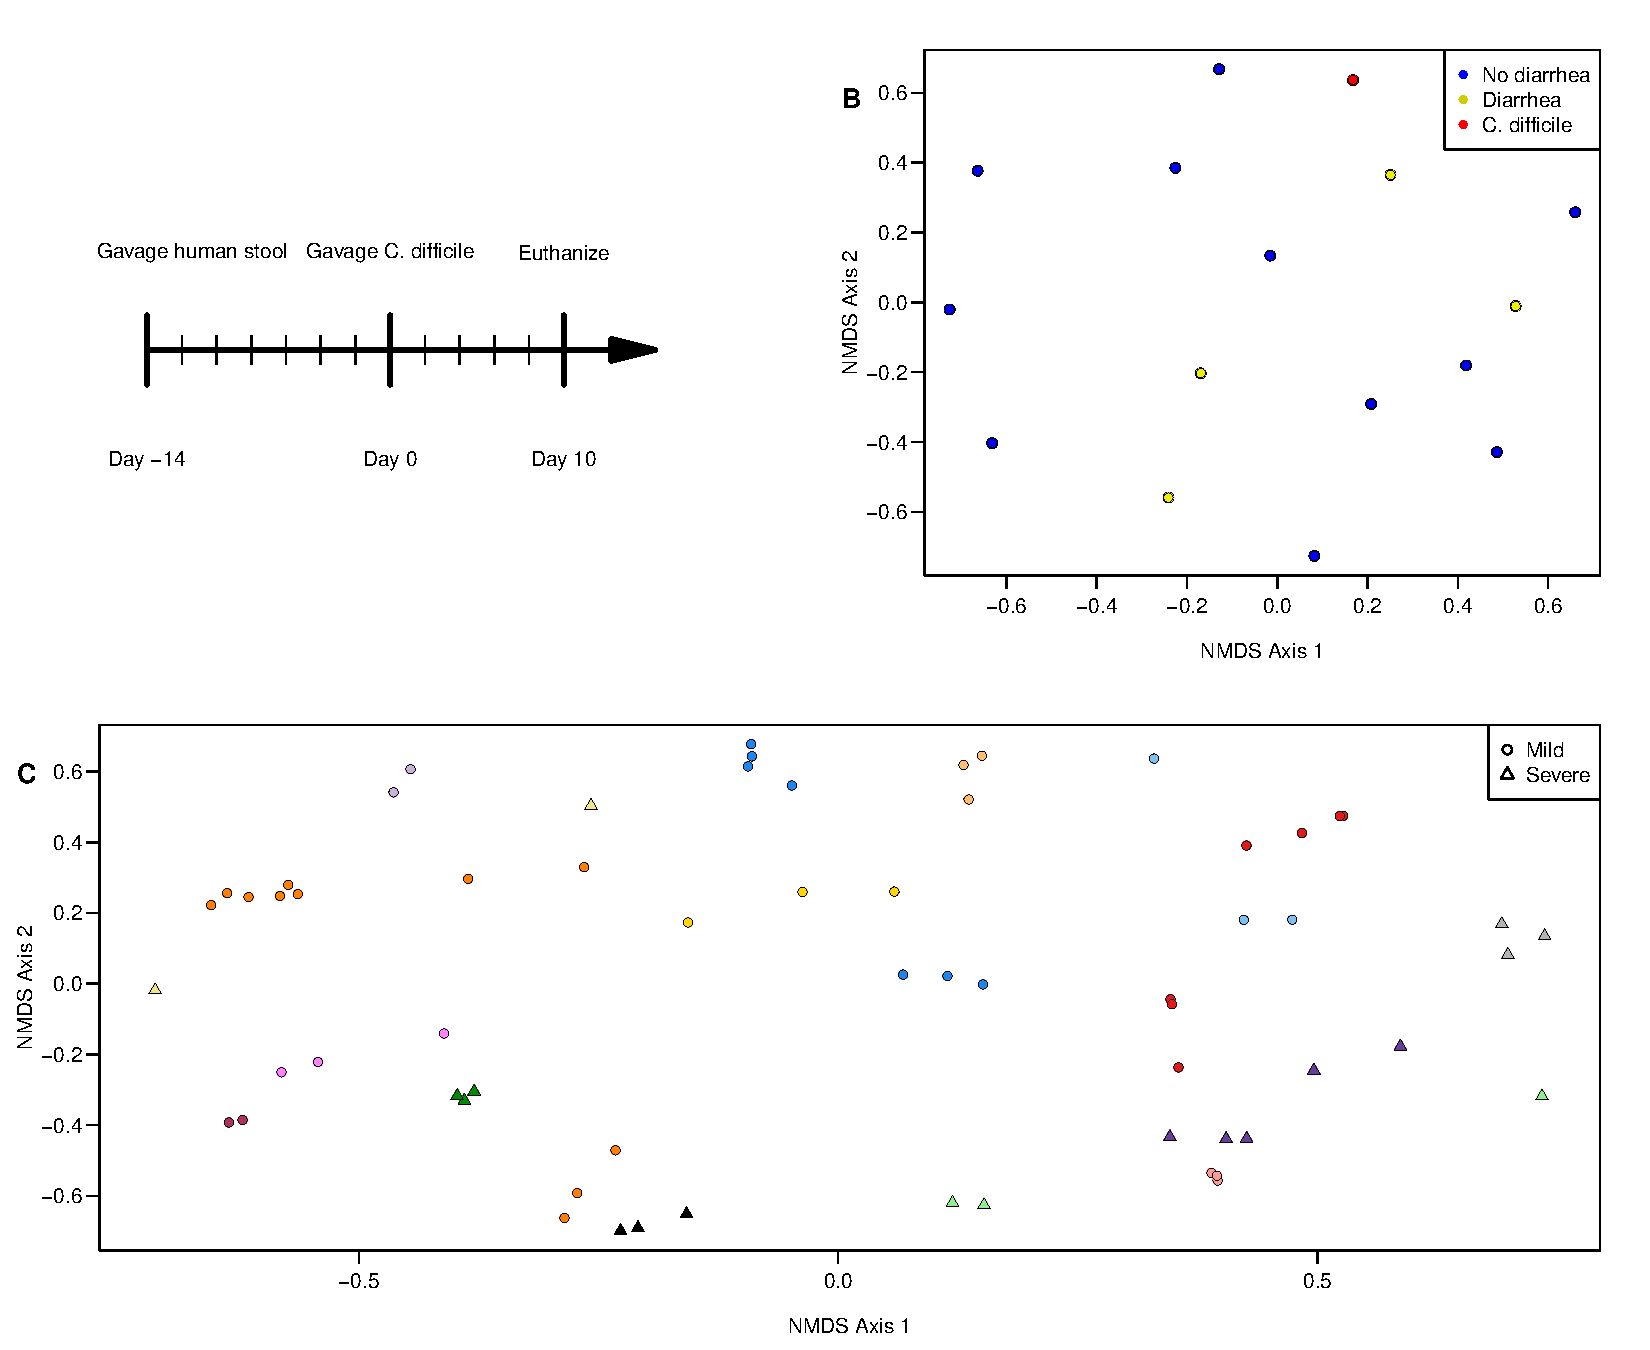
\includegraphics{../results/figures/figure_1.jpg}

\textbf{Figure 1. R.} (A-C).

\hfill\break

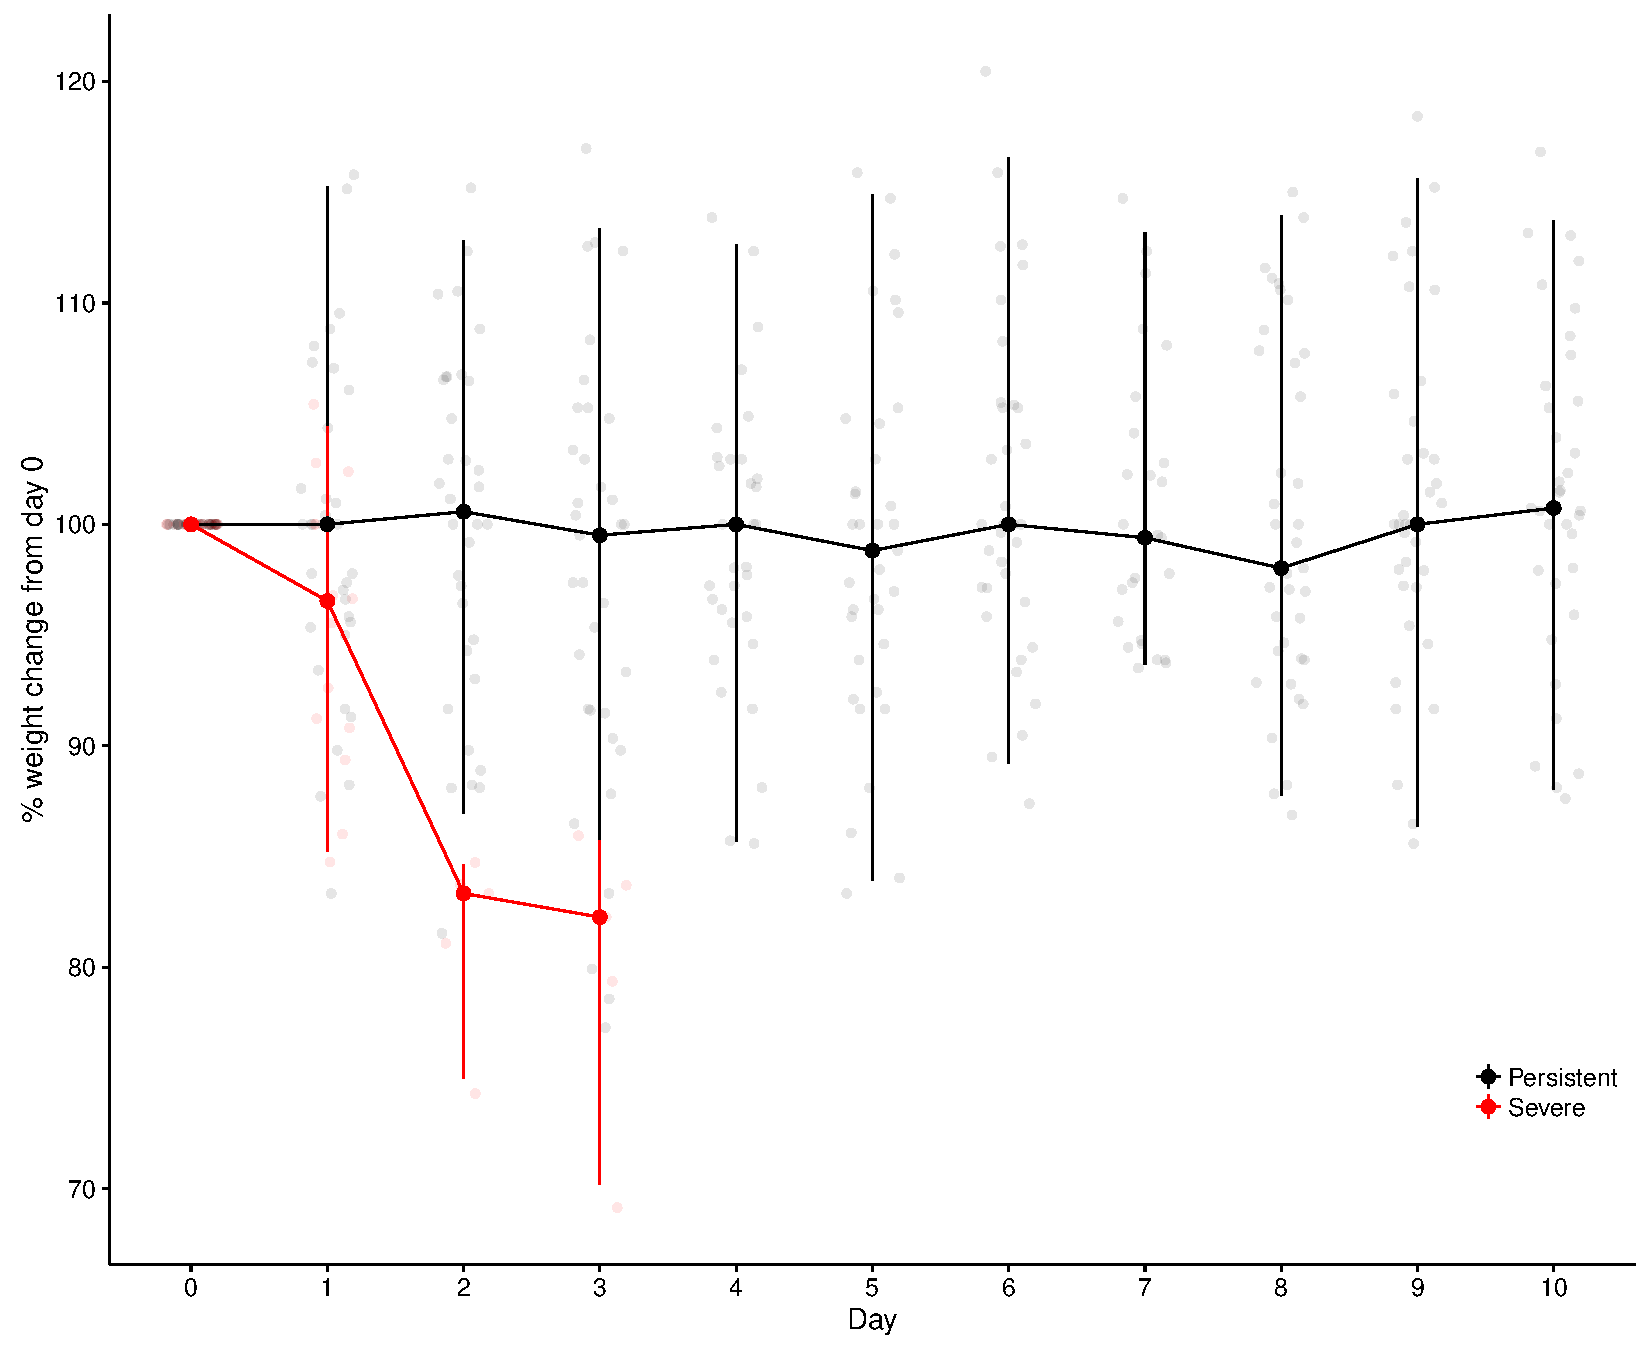
\includegraphics{../results/figures/figure_2.jpg}

\textbf{Figure 2. M.} F.

\hfill\break

\includegraphics{../results/figures/figure_3.jpg}

\textbf{Figure 3. O.} F.

\hfill\break

\includegraphics{../results/figures/figure_4.jpg}

\textbf{Figure 4. E.} A.

\hfill\break

\includegraphics{../results/figures/figure_5.jpg}

\textbf{Figure 5. D.} (A) L

\hfill\break

\includegraphics{../results/figures/figure_6.jpg}

\textbf{Figure 6. D.} (A) L

\hfill\break

\includegraphics{../results/figures/figure_S1.jpg}

\textbf{Figure S1. D.} (A) L

\hfill\break

\includegraphics{../results/figures/figure_S2.jpg}

\textbf{Figure S2. D.} (A) L

\hfill\break

\includegraphics{../results/figures/figure_S3.jpg}

\textbf{Figure S3. D.} (A) L

\hfill\break

\textbf{Table 1. D.} (A) L

samples\_used \textless-
readxl::read\_xlsx(`data/raw/humanGF\_ids.xlsx') \%\textgreater\%
pull(human\_source) \%\textgreater\% unique donor\_data \textless-
readxl::read\_xlsx(`data/raw/MIMARKS\_cdclinical.xlsx') \%\textgreater\%
filter(sample\_id \%in\% samples\_used) \%\textgreater\%
select(sample\_id, biome, age, gender, ``antibiotics \textgreater3mo'',
protonpump, antacid, Healthworker, historyCdiff, Surgery6mos,
Vegetarian, weight, disease\_stat)

\textbf{Table 2. D.} (A) L

read.csv(here(`data/raw/Hanna\_in\_vitro\_data\_plus\_germination.txt'))
\%\textgreater\% rownames\_to\_column(`isolate') \%\textgreater\%
filter(isolate \%in\% c(`DA00299', `DA00395', `DA00458', `DA00431'))

\end{document}
